 
\section{Modeling the photon detection efficiency}

The experimental variables influencing PDE are photon wavelength ($\lambda$), incidence angle ($\theta$), operating over-voltage ($V$) and to a lesser extent temperature ($T$). Operation in dense media modifies the PDE via optical coupling. We model the PDE using device specific parameters which describe a simplified PN junction\footnote{Naming conventions follow from \cite{gallina_avalanche_2019}. Junction depths are wrt the silicon surface.} and the avalanche triggering probabilities for the corresponding minority carriers. The SiPM surface is modeled as a thin silicon-dioxide layer, assumed sufficient for describing the efficiency of these devices where we infer a p-on-n junction structure. The model can be easily reversed for n-on-p devices. Simplified device structure is shown in \autoref{fig:pnSchematic}. Listed below are model parameters and some defined mathematical quantities:
% ------
% \begin{itemize}
%     \item $\lambda$ - photon wavelength
%     \item $\theta$ - incident photon angle in medium
%     \item $V$ - SiPM operating over-voltage
% \end{itemize}
% ------

% We use many mathematical or derived quantities.
% \begin{itemize}
%     \item $\bar{n} = n+ik$ - the complex refractive index, $k$ being the extinction coefficient
%     \item $\mu = \frac{4\pi k}{\lambda}$ - the attenuation coefficient, dependant on the extinction coefficient $k$
%     \item $\theta_{2, 3}$ - the photon's angle of incidence within the silicon dioxide (2) and bulk silicon (3), derived from
% \end{itemize}

\begin{itemize}[nosep]
    \item $\tox$ - average thickness of the surface silicon dioxide ($\ce{SiO2}$) passivation layer.
    \item $dp^*$ - effective depth representing top of p-doped region; below $dp^*$ electrons are collected and reach the high field region (near $X_{PN}$).
    \item $X_{PN}$ - the center of the p-n junction and location of high field region, boundary where avalanches are either e- or h+ driven.
    \item $dw^*$ - effective depth representing bottom of n-doped region; above $dw^*$ holes are collected and reach the high field region (near $X_{PN}$).
    \item $P_e(V), P_h(V)$ - probability a collected electron, hole triggers an avalanche. Empirically parameterized wrt voltage as $P_e(V;A_e, V_e) = A_e(1-e^{-\frac{V}{V_e}})$ and $P_h(V;A_h, V_h)=A_h(1-e^\frac{-V}{V_h})$.
    \item $FF$ - Fill Factor, fraction of photo-sensitive surface area.
    \item $\mathbf{J}$ - the set of device parameters listed above.
    \item $W_p, W_n$ - probability of photo-absorption within effective p, n regions.
    \item $T_{Si}$ - total probability of transmission into bulk silicon.
    \item $iPDE$ - the internal detection efficiency, efficiency of a photon in bulk silicon.
    \item $H$ - surface structure height $h$ relative to pixel pitch $p$ ($H = h/p$).
\end{itemize}

The PDE equation is factored into the separate terms: $FF$, transmission into silicon $T_{Si}$, and internal efficiency $iPDE$. Internal efficiency is given by the photoabsorption probability in the p (n) region $W_p$ ($W_n$) multiplied by the avalanche triggering probability of the corresponding minority carrier $P_e$ ($P_h$). The collection depths $dp^*$ and $dw^*$ include some diffusive contribution near the edges as described in \cite{gallina_avalanche_2019}; they are effective parameters correlated with the boundaries of the junction's depletion region. The PDE equation is written below with the first line omitting variables and parameters for clarity.
\begin{align}
    PDE & = FF \cdot T \cdot (P_e \cdot W_p + P_h \cdot W_n) \\
    \label{eq:PDE}
    PDE(\lambda, \theta, V; \mathbf{J}) & = FF \cdot T(\theta, \lambda; \tox) \cdot iPDE(V, \lambda; \mathbf{J}) \\
    iPDE(V, \lambda; \mathbf{J}) & = P_e(V) W_{p}(\lambda; dp^*, X_{PN}) + P_h(V) W_{n}(\lambda; X_{PN}, dw^*)
    \label{eq:iPDE}
\end{align}
To an excellent approximation the absorption functions $W_p, W_n$ are independent of incident photon angle $\theta$ due to strong refraction into silicon. The fill factor $FF$ is typically taken as constant, but for precision modeling can vary with surface structure, incident angle or wavelength (see \autoref{sec:ffTheta}, \cite{ACERBI2018_FF}).

\begin{figure}[h]
\centering
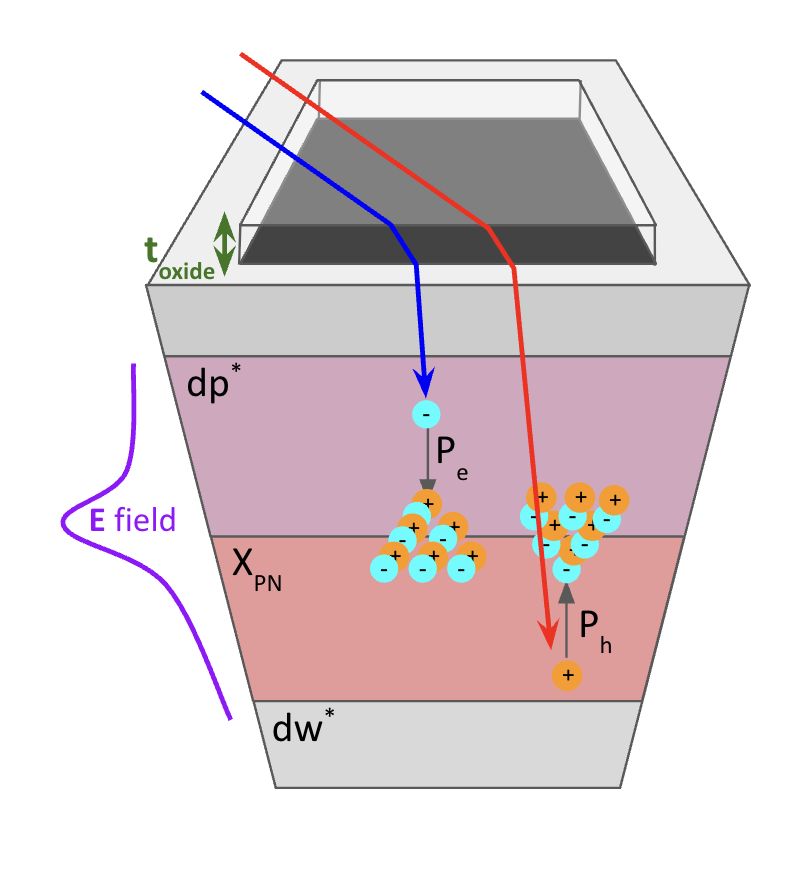
\includegraphics[width=.35\linewidth]{fig-diagram_v2.png}
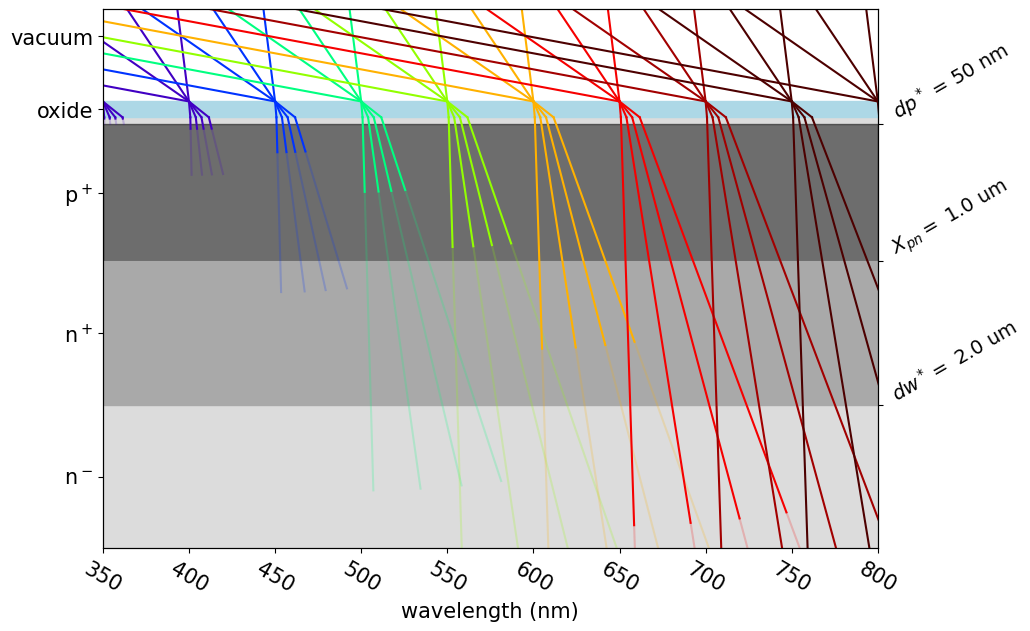
\includegraphics[width=.6\linewidth]{fig-schematic_ray_diagram_NOTITLE.png}
\caption{\label{fig:pnSchematic}
(Left) Diagram of the modeled SiPM structure, with illustration of the minority carriers drifting into the high field region and initiating avalanches. (Right) Ray diagram of photon paths in SiPM (for real part of internal angle $\theta_3$). Thick lines in silicon correspond to that wavelength's attenuation length $1/\mu$, with fainter lines drawn at length $4/\mu$. $n^-$ denotes the insensitive bulk silicon. The refracted angles are drawn accurately, highlighting the similarity in path length within silicon for different angles of incidence.}
\end{figure}

\subsection{Input optical data}
\label{sec:inputOpticalData}

\begin{figure}[htbp]
\centering
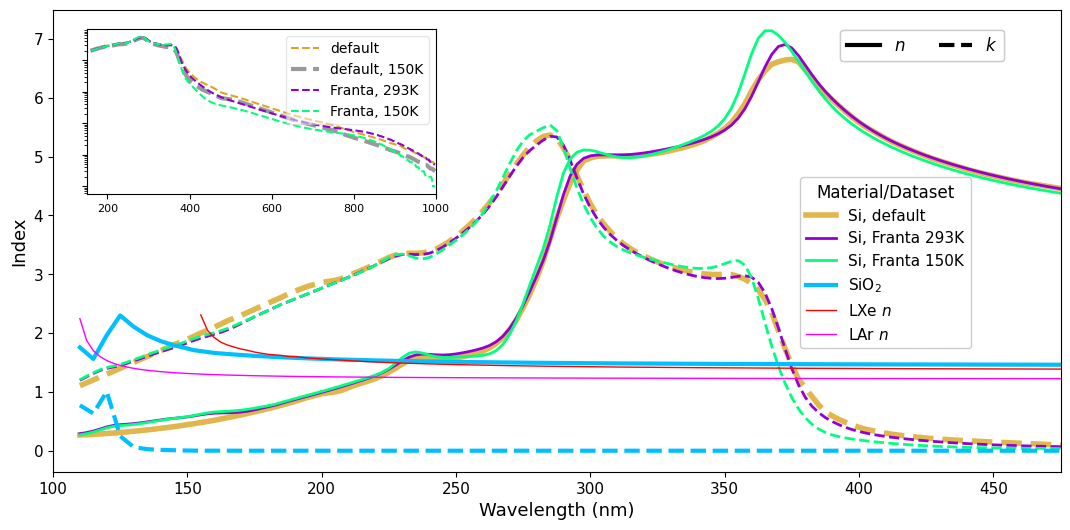
\includegraphics[width=.9\linewidth]{fig-inputData_v2.png}
       
  \caption{\label{fig:input_data} The input optical data used in this work. Solid and dashed lines represent $n$ and $k$, respectively (main figure).  All silicon $n$ values asymptote to $\sim$3.55 at 1000~nm. Inset figure shows Vis-IR $k$ values on a log scale; the differences between these curves drive variation in fit results due to different photoabsorption. The thicker gray `default, 150~K' $k$ curve under the purple line is the default data scaled by the photoabsorption model. Data references are given in the text. The liquid nobles $n$ values are drawn above where $k = 0$.}
\end{figure}

The complex refractive indices $(n, k)$ of silicon, $\sio$ and the detection media are fixed inputs to the model for calculating $T_{Si}$ and $W_p, W_n$. To cover the wavelength range of interest, $\sio$ data was combined from \cite{lithography} over 110-800~nm \footnote{dataset with $k=0$ at $\sim$160~nm selected for consistency with known VUV PDE} and \cite{Malitson} deeper into the IR\footnote{Datasets merged and smoothed in 50~nm region of overlap where datasets had small disagreement}. The $n$ and $k$ data for pure silicon were combined from \cite{lithography} in the VUV (110-200~nm), \cite{nSi_aspnes} (200-750~nm) for UV-Vis\footnote{this dataset is considered more reliable than \cite{nSi_schinke}, which exhibited shape inconsistent with precision Franta dataset \cite{nSi_franta_full_2017} and yielded poorer fit quality} and \cite{nSi_schinke} into the IR. This is referred to as the `default' silicon dataset and used throughout, unless otherwise noted. Curves for ultrapure `float zone' silicon at 150~K are taken from \cite{nSi_franta_full_2017}, which presents a complex theoretical model yielding $n$ and $k$ as a function of silicon purity and temperature\footnote{values taken from \url{https://refractiveindex.info/}}. These values are referred to hereafter as the `Franta' dataset, which are used to investigate model variability with input optical data.

% Some ad-hoc data selection was required; for $\sio$ we chose the dataset from \cite{lithography} with $k=0$ until $\sim$160~nm, consistent with measured VUV PDE and expectation of transparency to LXe scintillation light. For the default $\si$ data, we consider the dataset from \cite{nSi_aspnes} to be more reliable than an alternative dataset from \cite{nSi_schinke}, which exhibited a shape inconsistent with the higher-precision Franta dataset and yielded an overall poorer fit quality.

Input optical data is plotted in \autoref{fig:input_data}, including LXe data from \cite{excitonicBands_lxe_laporte_1977}, \cite{lxe_n_sinnockSmith} and LAr data from \cite{lar_lxe_GRACE2017}. Using pure silicon optical data makes the simplifying assumption that modifications to $n, k$ due to dopants are negligible, avoiding the complexity of including and estimating doping profiles. This assumption is revisited in \autoref{sec:discussion}, as usage of the Franta dataset (with lower $k$ in the NIR) significantly modifies fit parameters. A photoabsorption temperature correction, described in \autoref{model:temp}, does not reduce the room temperature $k$ values of the default dataset as low as the theoretically derived Franta values.

\subsection{Transmittance and reflectivity}
Transmission is modeled as bulk silicon ($\si$) with a thin silicon-dioxide ($\sio$) surface layer, following from the success of this approach in fitting SiPM reflectivity\cite{sipmRef_nexo_guofu}. The vacuum-$\sio$-$\si$ layers are labeled with subscript $1, 2, 3$ respectively. The complex refraction angles in the oxide $\theta_2$ and silicon $\theta_3$ are calculated with Snell's law. \autoref{eq:transmission} is the wave-optics derived transmission from region 1 to 3 for a two interface system with film thickness $\tox$ \cite{kurtis_thesis}, which differs for S($\perp$) or P($\parallel$) polarized photons. $r_{i,j}$, $t_{i,j}$ are the Fresnel coefficients from medium $i$ to $j$. The phase change due to interference within the thin film is given by $\delta$, which drives the oscillatory behavior of $T$ and includes possibly attenuation within the $\sio$. 
\begin{align}
    T_{13, \parallel or \perp} (\lambda, \theta; \tox) &= \frac{\Re (n_3 \cos\theta_3)}{\Re (n_1 \cos\theta_1)} \Big| \frac{t_{12}t_{23}e^{i\delta}}{1 + r_{12}r_{23}e^{i2\delta}} \Big|^2  _{\parallel or \perp}     \label{eq:transmission} \\
    \delta &= 2\pi \frac{n_2 t_{ox}}{\lambda}\cos\theta_2 \\
    T_{Si} &= \nicefrac{1}{2}(T_{13,\parallel} + T_{13, \perp})
\end{align}
The two polarizations are averaged yielding transmission into silicon $T_{Si}$. A similar expression for reflectivity \autoref{eq:Ref_wave} is used for analyzing reflectivity data, where for UV light we assume specular reflectivity from only the active silicon region; $R_{SiPM} \approx FF_o \cdot R_{Si}$. Transmission curves are shown in \autoref{fig:trans_and_abs} and contrasted with the classical ray-optics result. The inset plot shows effects of VUV light absorption in the $\sio$ layer.
\begin{equation}
    R_{13, \parallel or \perp} (\lambda, \theta; \tox)= |\frac{r_{12} + r_{23} e^{i \delta}}{1 + r_{12} r_{23} e^{i \delta}} |^2_{\parallel or \perp}
    \label{eq:Ref_wave}
\end{equation}

% \footnote{the complex valued refractive index is input while only the real component of the resulting angle is kept. The resulting imaginary angle represents the surface of constant amplitude, not constant phase.}

%% Poynting paragraph
An important distinction must be made for P-polarized light at oblique incidence on lossy media such as silicon. In this scenario, the Fresnel field equations predict $T+R < 1.0$. This `missing' Fresnel fraction is typically attributed to absorption within a skin layer, which may contribute to the UV PDE signal. Using the Poynting vector to calculate the transmission retains $R + T = 1.0$ with the direction of energy flow bent further towards the normal than $\Re (\theta_3)$. To account for this, at oblique incidence above 160~nm $T_{Si} = 1-R_{Si}$ is used as \autoref{eq:Ref_wave} is valid over all angular phase space. For oblique angles and $\lambda < 160$~nm, where absorption occurs in the quartz film, disentangling the missing Fresnel fraction from absorption in $\sio$ is less straightforward; using \autoref{eq:transmission} with $\Re ({\theta_3})$ is a good approximation but not exact.
%\autoref{eq:transmission} is valid for normal incidence.

The VUV4 device has a thick quartz window. Fresnel's equations and \sio data is used to calculate the window's transmission and reflectivity $T_W$ and $R_W$, which are combined with $T_{Si}$ and $R_{Si}$ by geometric series giving the total transmission for the system.
\begin{equation}
    \label{eq:T_total}
    T_{total} = \frac{T_W T_{Si}}{1 - R_{Si}R_W}
\end{equation}

\subsection{Internal PDE}
\label{sec:internal_pde}
Upon entering silicon a photon can be absorbed in the `dead region'\footnote{so-called because it is assumed photo-generated carriers produced close to the device surface are lost due to recombination} from $0<z<dp^*$, the effective $p$-doped region $dp^*<z<X_{PN}$, effective $n$-doped region $X_{PN}<z<dw^*$ or the insensitive bulk $z > dw^*$. This treatment assumes perfect collection efficiency within these regions and zero outside, and may be referred to as the `hard-edge' model. Silicon absorption length $\mu$ is calculated from the imaginary part of the refractive index.
\begin{equation}
\mu(\lambda; k) = 4 \pi\frac{k}{\lambda}
\label{eq:k_to_mu}
\end{equation}
Photon path lengths are calculated using the real internal angle $\Re(\theta_3)$. Absorption weights for each region, $W_p$ and $W_n$, are the integral over the region scaled by the attenuation prior to (\autoref{eq:w_values}). Curves in \autoref{fig:trans_and_abs} illustrate the effect of different junction geometries; shallower $dp^*$ improves UV absorption, a deeper high-field region $X_{PN}$ shifts the tradeoff between electron or hole driven avalanches, and larger junction ($dw^*$) increases NIR absorption. Due to the strong refraction or `lensing' into the silicon, the $W$ values have negligible dependence on $\theta_1$ over the phase space where transmission remains significant; a NIR photon (least refracted) incident at $80^o$ will have an internal angle of $\sim 20^o$ in bulk. As such $\theta$ dependence is omitted from the internal efficiency $iPDE$.
\begin{align}
    \label{eq:w_values}
    W_p(\lambda, \theta_3; dp^*, X_{PN}) &= e^{-\mu \cdot dp^* / \cos\theta_3}(1-e^{-\mu (X_{PN} - dp^*))/\cos\theta_3}) \\
    W_n(\lambda, \theta_3; X_{PN}, dw^*) &= e^{-\mu \cdot X_{PN} / \cos\theta_3}(1-e^{-\mu (dw^* - X_{PN})/\cos\theta_3})
\end{align}

\begin{figure}[htbp]
\centering
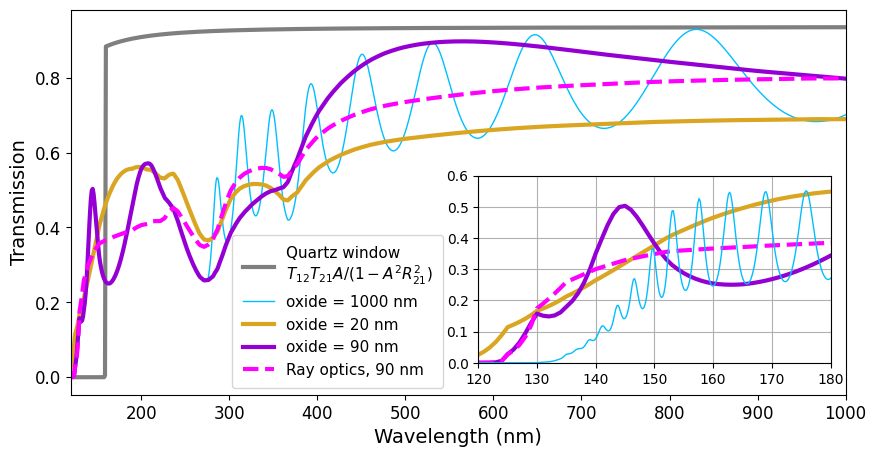
\includegraphics[width=.52\linewidth]{fig-transmission_wInset-font.png}
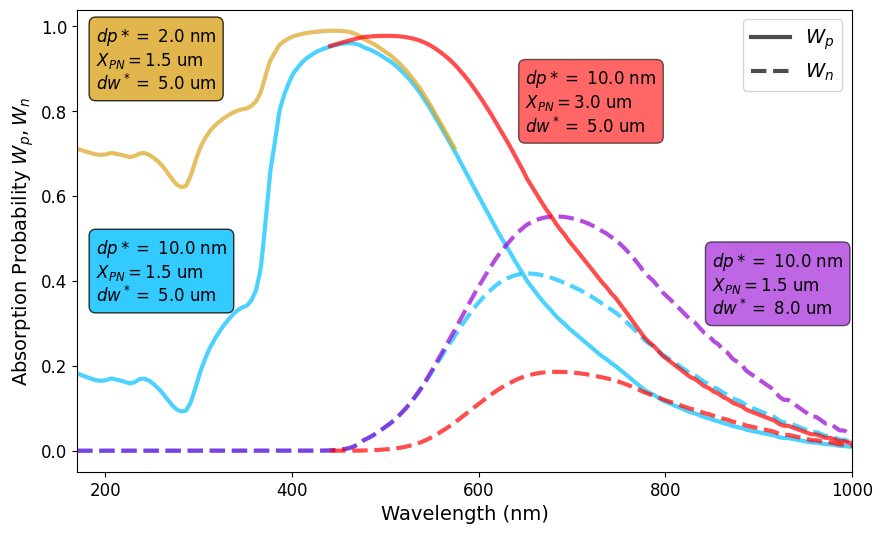
\includegraphics[width=.47\linewidth]{fig-W_absorption-font.png}

\caption{\label{fig:trans_and_abs} (Left) Vacuum transmission for the vacuum-quartz-silicon thin film interface in the PDE model. The dashed pink line is the transmission for ray optics; the thin-film transmission (using \autoref{eq:transmission}) oscillates about this mean value. The 20~nm thick (gold) curve is interference-enhanced below 300~nm while the thicker 90~nm curve (purple) oscillates in the VUV and is constructive above 380~nm. The 1$\um$ oxide oscillates rapidly for monochromatic light, and is truncated in VUV for clarity. Inset graph shows the region of interest for liquid noble applications. (Right) Absorption probability vs wavelength for electron ($W_p$, solid) and hole ($W_n$, dashed) collection regions. The different curves highlight the influence of PN geometry.}

\end{figure}

% \caption{\label{fig:trans_and_abs} Absorption probability vs wavelength for the electron collection region $W_p$ (solid lines) and hole collection region $W_n$ (dashed). The different curves highlight the following influence of PN geometry: proximity to surface ($dp^*$) improves absorption in the UV, a deeper high-field region $X_{PN}$ shifts the tradeoff between electron or hole driven avalanches, and deeper junction ($dw^*$) increases absorption for NIR wavelengths.}

Building upon the study of avalanche triggering probabilities \cite{gallina_avalanche_2019, Zappala_2016_efficiency}, $iPDE$ is given by multiplying the absorption weights by their corresponding minority carrier's avalanche probability, $iPDE = P_e \cdot W_p + P_h \cdot W_n$. This convenient form arises from the assumption that electrons (holes) generated anywhere within the effective p-region (n-region) are successfully drifted to the high-field region about $X_{PN}$ where avalanches are initiated\cite{oldham_avalanche, mcintyre_new_1999} \footnote{defined as the region where impact ionization of both $e^-$ and $h^+$ is above threshold}. The sharp transition from $P_e$ to $P_h$ about $X_{PN}$ stems from the simplification that the high-field region is small relative to the photon absorption scale\footnote{Physically there is a small volume where photo-generated e/h pairs have an avalanche probability somewhere between $P_e$ and $P_h$, as \textit{both} charge carriers pass through a fraction of their respective avalanche inducing regions \cite{chaves_2021_analyticAvalanche}.}. Avalanche efficiency is described with the empirical parameterization $P_e(V) = A_e\cdot(1-e^{-V/V_e})$ and similarly for $P_h$, as demonstrated in \cite{Lewis_2025_qy,Zappala_2016_efficiency}. Later we show $A_e$ can be fixed to 1.0 for the devices studied here. As VUV light generates multiple e-h pairs the $P_e$ term becomes a function of photon energy through the quantum yield $\eta(\lambda) > 1$ \cite{Lewis_2025_qy} . The $P_e$ term then follows binomial statistics $P_e(\lambda) \rightarrow 1 - (1-P_e)^\eta(\lambda)$. 

\subsection{Fill factor and angular dependence}
\label{sec:ffTheta}
The fill factor $FF$ represents the fraction of the SiPM surface sensitive to incident photons. Design elements such as the quenching resistors surrounding each SPAD contribute to the insensitive fraction $1-FF$. For most applications, $FF$ may be treated as a fixed value independent of angle of incidence (AOI) or wavelength. However border effects within bulk modify the electric field near SPAD edges, resulting in possible wavelength dependence of $FF$ \cite{ACERBI2018_FF} for different absorption depths. Large resistor heights relative to SPAD size can shadow the active area effectively reducing $FF$ for oblique incidence. To build a shadowing model, we simplify the geometry and treat the insensitive region as a symmetric, raised square loop surrounding the SPAD. With $p$ the known SPAD pitch, the one dimensional resistor width $ff$ can be calculated from the ratio of sensitive area to total area for a SPAD, $FF = \frac{(p-2ff)^2}{p^2}$. 

Assuming the resistor material is not reflective, for incident light in a plane perpendicular to the resistor the shadowed area is calculated. With a barrier of height $h$ and light at incidence angle $\theta$, the shadow length $h\tan\theta$ is multiplied by the sensitive region's side length $p-2ff$. Defining the relative resistor width $W\equiv ff/p$ and height $H\equiv h/p$, the shadowed fill factor can be written as below, with $FF_o$ the fill factor at normal incidence. In \autoref{sec:fitting_the_model} this model is fit to angular PDE data for the Hamamatsu VUV4 and compared to AFM measurements.
\begin{equation}
    FF(\theta) = F_o - \frac{(p-2ff)h}{p^2}\tan\theta = FF_o - (1-2W)H\tan\theta
    \label{eq-FFtheta}
\end{equation}

\subsection{Temperature and Photoabsorption}
\label{model:temp}
Operating temperature impacts PDE via different mechanisms; modified optics, photoabsorption, carrier mobility and carrier freezeout. Non-monotonic variation in PDE with respect to temperature has been measured, with inflection points at $\sim$150~K \cite{biroth_icasipm_2018} and $\sim$ 200~K \cite{sipm_temp_pde_collazuol_2011}. Studies of a thin device in \cite{acerbi_2023} show further variance of inflection point location and monotonicity depending on wavelength and bias voltage. Negligible temperature respons is reported at 450 nm in \cite{cryogenic_2025_rivera}, and between 160 K and room temperature at 175 nm in vacuum \cite{gallina_performance_2022}. Narrowband studies \cite{garrote_2024_cryoPDE, Wang_2021_cryo_sCurve, Borden_pdeTemp_2024, gu_2025_heliumPDE,PKLightfoot_2008} show varied response. Clearly temperature dependence is wavelength and device dependent. We add a simple extension to the PDE model by including the temperature dependence of photo-absorption for bulk silicon, the expected dominant mechanism for Vis-IR light at temperatures above carrier freezeout. Transmission was minimally impacted when comparing results using the warm or cryogenic $n, k$ input datasets. Carrier freezeout occurs at approximately $\sim 100$~K \cite{biroth_2015_cryogenic}, below the range studied here. A recovery in charge collection efficiency at very low temperatures is the suggested mechanism allowing non-zero PDE at 4~K, which counteracts freezeout effects \cite{biroth_2015_cryogenic, cce_cryogenic_1998}.

% For indirect bandgap materials, photoabsorption decreases with temperature due to both the decrease in phonon population and the increase in the bandgap energy.
As silicon's two lowest bandgaps (1.15, 2.25 eV) are indirect, photoabsorption is strongly temperature dependent from the IR until the direct bandgap at $\sim$ 380~nm (3.4~eV). In \cite{siBandgap_dmPaper} the absorption coefficient $\alpha(\lambda, T) \equiv 1/\mu$ was parameterized in silicon over 440-1000~nm from 4-300~K, for applications in low mass DM searches. We replace the direct bandgap description in \cite{siBandgap_dmPaper} (taken from \cite{siBandgap_solarCells}, \cite{siBandgap_cardona_1985}) with that from \cite{siAbsorption_Bucher} for consistency with photoabsorption values calculated from $k$ data.
% When transforming the parameterized $\alpha$ to $k$ using equation \ref{eq:k_to_mu}, the resonance about 360~nm is not present. Due to this lack of structure, and the systematically low attenuation lengths and sparse wavelength measurements in \cite{siBandgap_dmPaper}, 
To retain the wavelength structure in $k$, which is absent from the sparse data of \cite{siBandgap_dmPaper}, we use the parameterization to calculate the relative change to $\mu(\lambda, T)$ derived from the default $k$ dataset\footnote{Numerical smoothing is done about the direct bandgap threshold where a discontinuity arises. The functional form in selected from \cite{siAbsorption_Bucher} also reduces the discontinuity about this point compared to other functions}. The result is the temperature dependence for photoabsorption in silicon, with $\alpha(\lambda, T)$ the modified form from \cite{siBandgap_dmPaper}:
\begin{equation}
    \mu(\lambda, T; k) = \mu_o(\lambda; k) \frac{\alpha(\lambda, T=300\text{K})}{\alpha(\lambda, T)}
    \label{eq:alpha_relative}
\end{equation}